\documentclass{article}\usepackage[]{graphicx}\usepackage[]{color}
%% maxwidth is the original width if it is less than linewidth
%% otherwise use linewidth (to make sure the graphics do not exceed the margin)
\makeatletter
\def\maxwidth{ %
  \ifdim\Gin@nat@width>\linewidth
    \linewidth
  \else
    \Gin@nat@width
  \fi
}
\makeatother

\definecolor{fgcolor}{rgb}{0.345, 0.345, 0.345}
\newcommand{\hlnum}[1]{\textcolor[rgb]{0.686,0.059,0.569}{#1}}%
\newcommand{\hlstr}[1]{\textcolor[rgb]{0.192,0.494,0.8}{#1}}%
\newcommand{\hlcom}[1]{\textcolor[rgb]{0.678,0.584,0.686}{\textit{#1}}}%
\newcommand{\hlopt}[1]{\textcolor[rgb]{0,0,0}{#1}}%
\newcommand{\hlstd}[1]{\textcolor[rgb]{0.345,0.345,0.345}{#1}}%
\newcommand{\hlkwa}[1]{\textcolor[rgb]{0.161,0.373,0.58}{\textbf{#1}}}%
\newcommand{\hlkwb}[1]{\textcolor[rgb]{0.69,0.353,0.396}{#1}}%
\newcommand{\hlkwc}[1]{\textcolor[rgb]{0.333,0.667,0.333}{#1}}%
\newcommand{\hlkwd}[1]{\textcolor[rgb]{0.737,0.353,0.396}{\textbf{#1}}}%
\let\hlipl\hlkwb

\usepackage{framed}
\makeatletter
\newenvironment{kframe}{%
 \def\at@end@of@kframe{}%
 \ifinner\ifhmode%
  \def\at@end@of@kframe{\end{minipage}}%
  \begin{minipage}{\columnwidth}%
 \fi\fi%
 \def\FrameCommand##1{\hskip\@totalleftmargin \hskip-\fboxsep
 \colorbox{shadecolor}{##1}\hskip-\fboxsep
     % There is no \\@totalrightmargin, so:
     \hskip-\linewidth \hskip-\@totalleftmargin \hskip\columnwidth}%
 \MakeFramed {\advance\hsize-\width
   \@totalleftmargin\z@ \linewidth\hsize
   \@setminipage}}%
 {\par\unskip\endMakeFramed%
 \at@end@of@kframe}
\makeatother

\definecolor{shadecolor}{rgb}{.97, .97, .97}
\definecolor{messagecolor}{rgb}{0, 0, 0}
\definecolor{warningcolor}{rgb}{1, 0, 1}
\definecolor{errorcolor}{rgb}{1, 0, 0}
\newenvironment{knitrout}{}{} % an empty environment to be redefined in TeX

\usepackage{alltt}
\usepackage{natbib}
\IfFileExists{upquote.sty}{\usepackage{upquote}}{}
\begin{document}

\title{The Shunned House Wordcloud}
\author{Andrew Innes}
\maketitle

\begin{abstract}
In this article we construct a wordcloud, using the tidytext R package, for H.P. Lovecraft's The Shunned House.

\end{abstract}

\textit{The Shunned House} is a horror fiction novelette by American author H.P. Lovecraft, published in 1937\footnote{The novel was published in the October 1937 issue of Weird Tales.}.  Below we craft a wordcloud for the most common words appearing in the novelette.

\section{The Gutenberg Package}
The Gutenberg Package is a package for R, gutenbergr, that gives one access to the books in Project Gutenberg.  One has to first install this package and bring it in with library.  You may then call the following function and store the result.  Since we will be using The Shunned House we will download it using its unique integer identifier.  In order to do this we must execute the following code:

\begin{knitrout}
\definecolor{shadecolor}{rgb}{0.969, 0.969, 0.969}\color{fgcolor}\begin{kframe}
\begin{alltt}
\hlkwd{library}\hlstd{(gutenbergr)}
\hlkwd{library}\hlstd{(stringr)}
\hlkwd{gutenberg_works}\hlstd{(}\hlkwd{str_detect}\hlstd{(title,}\hlstr{'The Shunned House'}\hlstd{))}
\end{alltt}
\begin{verbatim}
## # A tibble: 1 x 8
##   gutenberg_id             title                             author
##          <int>             <chr>                              <chr>
## 1        31469 The Shunned House Lovecraft, H. P. (Howard Phillips)
## # ... with 5 more variables: gutenberg_author_id <int>, language <chr>,
## #   gutenberg_bookshelf <chr>, rights <chr>, has_text <lgl>
\end{verbatim}
\begin{alltt}
\hlstd{House}\hlkwb{<-}\hlkwd{gutenberg_download}\hlstd{(}\hlnum{31469}\hlstd{)}

\hlstd{House}
\end{alltt}
\begin{verbatim}
## # A tibble: 1,065 x 2
##    gutenberg_id
##           <int>
##  1        31469
##  2        31469
##  3        31469
##  4        31469
##  5        31469
##  6        31469
##  7        31469
##  8        31469
##  9        31469
## 10        31469
## # ... with 1,055 more rows, and 1 more variables: text <chr>
\end{verbatim}
\end{kframe}
\end{knitrout}

This dataframe has two columns, one for the The ID Number of the book, and one containing the text from the book. Now we are ready for very litte data cleaning.

\section{Very Little Data Cleaning}

We would like to remove the front matter of the book.  By inspection, we have determined that the front matter ends on line 6.  Therefore we can redefine House to begin on line 7:

\begin{knitrout}
\definecolor{shadecolor}{rgb}{0.969, 0.969, 0.969}\color{fgcolor}\begin{kframe}
\begin{alltt}
\hlkwd{library}\hlstd{(dplyr)}
\hlstd{House}\hlkwb{<-}\hlstd{House[}\hlnum{7}\hlopt{:}\hlnum{1055}\hlstd{,]}
\end{alltt}
\end{kframe}
\end{knitrout}

\section{The Wordcloud}

To make the wordcloud, we first have to break up the lines into words.  We can use a function from the tidytext package for this:

\begin{knitrout}
\definecolor{shadecolor}{rgb}{0.969, 0.969, 0.969}\color{fgcolor}\begin{kframe}
\begin{alltt}
\hlkwd{library}\hlstd{(tidytext)}
\hlstd{words_df}\hlkwb{<-}\hlstd{House}\hlopt
  \hlkwd{unnest_tokens}\hlstd{(word,text)}

\hlstd{words_df}
\end{alltt}
\begin{verbatim}
## # A tibble: 10,968 x 2
##    gutenberg_id       word
##           <int>      <chr>
##  1        31469         _a
##  2        31469 posthumous
##  3        31469      story
##  4        31469         of
##  5        31469    immense
##  6        31469      power
##  7        31469    written
##  8        31469         by
##  9        31469          a
## 10        31469     master
## # ... with 10,958 more rows
\end{verbatim}
\end{kframe}
\end{knitrout}

We can remove the common, unimportant words with the stop\_words data frame and some dplyr:

\begin{knitrout}
\definecolor{shadecolor}{rgb}{0.969, 0.969, 0.969}\color{fgcolor}\begin{kframe}
\begin{alltt}
\hlstd{words_df}\hlkwb{<-}\hlstd{words_df}\hlopt
  \hlkwd{filter}\hlstd{(}\hlopt{!}\hlstd{(word} \hlopt \hlstd{stop_words}\hlopt{$}\hlstd{word))}

\hlstd{words_df}
\end{alltt}
\begin{verbatim}
## # A tibble: 4,547 x 2
##    gutenberg_id       word
##           <int>      <chr>
##  1        31469         _a
##  2        31469 posthumous
##  3        31469      story
##  4        31469    immense
##  5        31469      power
##  6        31469    written
##  7        31469     master
##  8        31469      weird
##  9        31469    fiction
## 10        31469       tale
## # ... with 4,537 more rows
\end{verbatim}
\end{kframe}
\end{knitrout}

Now, we need to calculate the frequencies of the words in the novelette.  Again, we can use standard dplyr techniques for this:

\begin{knitrout}
\definecolor{shadecolor}{rgb}{0.969, 0.969, 0.969}\color{fgcolor}\begin{kframe}
\begin{alltt}
\hlstd{word_freq}\hlkwb{<-}\hlstd{words_df}\hlopt
  \hlkwd{group_by}\hlstd{(word)}\hlopt
  \hlkwd{summarize}\hlstd{(}\hlkwc{count}\hlstd{=}\hlkwd{n}\hlstd{())}

\hlstd{word_freq}
\end{alltt}
\begin{verbatim}
## # A tibble: 2,652 x 2
##           word count
##          <chr> <int>
##  1          _a     1
##  2    _cellar_     1
##  3      _daily     1
##  4     _elbow_     1
##  5 _emanation_     1
##  6    _gaspee_     1
##  7       _had_     1
##  8         _in     1
##  9    _jacques     1
## 10 _providence     1
## # ... with 2,642 more rows
\end{verbatim}
\end{kframe}
\end{knitrout}

Finally, it's time to generate the wordcloud:

\begin{knitrout}
\definecolor{shadecolor}{rgb}{0.969, 0.969, 0.969}\color{fgcolor}\begin{kframe}
\begin{alltt}
\hlkwd{library}\hlstd{(wordcloud)}
\hlkwd{wordcloud}\hlstd{(word_freq}\hlopt{$}\hlstd{word,word_freq}\hlopt{$}\hlstd{count,}\hlkwc{min.freq} \hlstd{=} \hlnum{5}\hlstd{)}
\end{alltt}
\end{kframe}
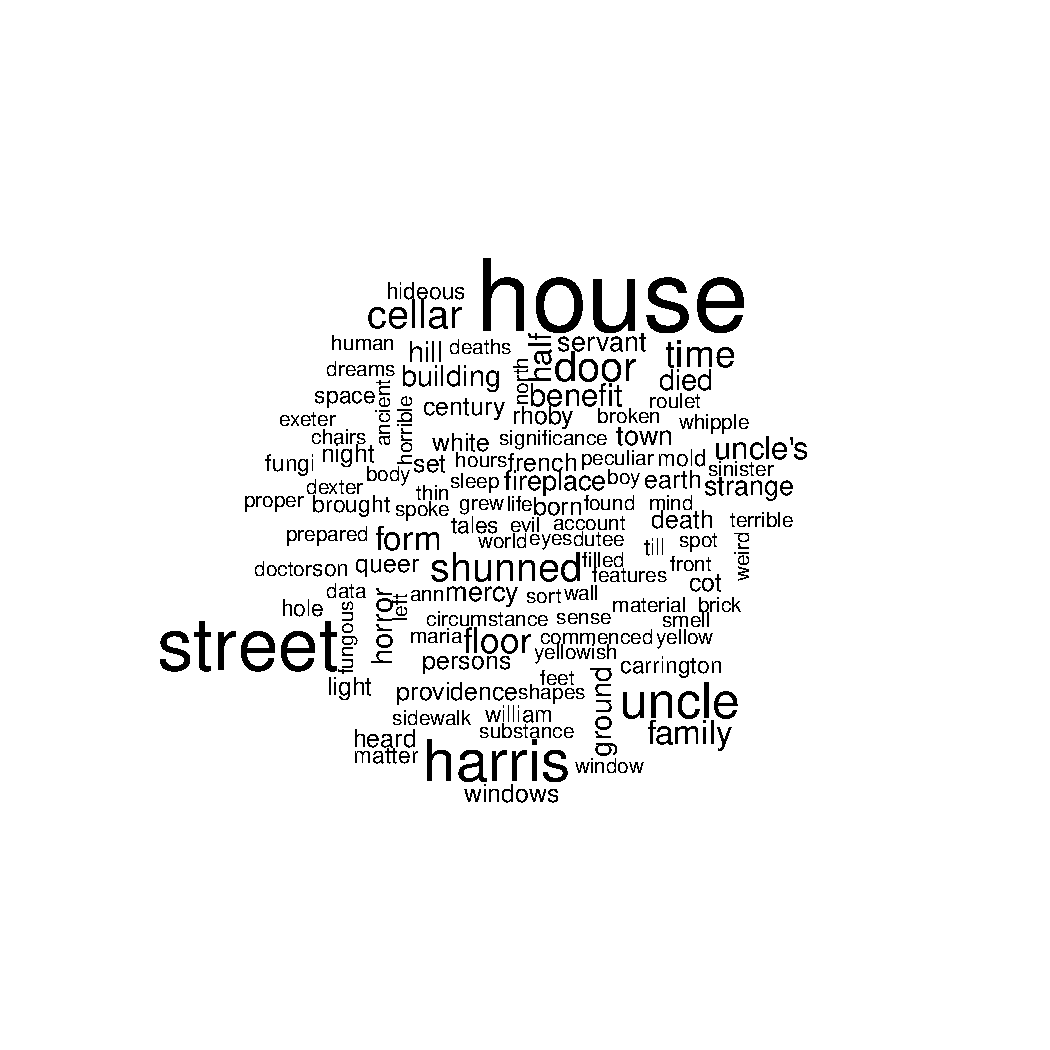
\includegraphics[width=\maxwidth]{figure/unnamed-chunk-6-1} 

\end{knitrout}

\bibliographystyle{apa}
\bibliography{Halloween_Article}
\nocite{*}

\end{document}
